\documentclass[12pt,]{article}
\usepackage{graphicx}
\usepackage{subcaption}
\usepackage{float}
\graphicspath{{Images/}}
\usepackage{amsmath}
%\usepackage{wrapfig}

\begin{document}
\section*{Raspberry Pi 3}
\textbf{Installing Debian Jessie set-up}\\
First Win32DiskImager has to be installed. Prior to the installation insert a micro SD into an USB adaptor and plug it into the computer.
Double click the win32diskimager-1.0.0-install.exe located in /Instalation Files and Required Software and a window will pop up as show on figure~\ref{fig:1}. Accept the license agreement and select "Next".
\begin{figure}[H]
  	\begin{center}
    	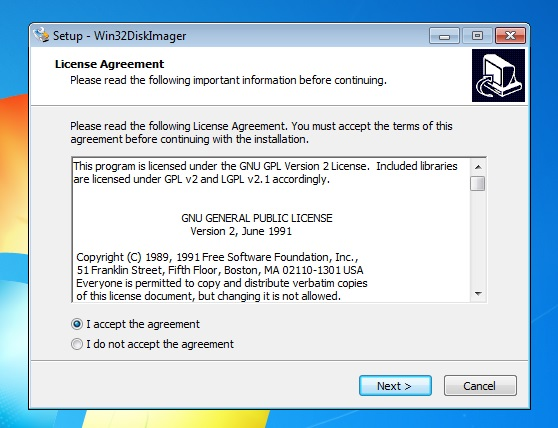
\includegraphics[width=0.5\textwidth]{Win32_1}
  	\end{center}
  	\caption{Win32DiskImager installation process part 1}
	\label{fig:1}
\end{figure}
Next on figure~\ref{fig:2} choose the installation directory and select "Next".
\begin{figure}[H]
  	\begin{center}
    	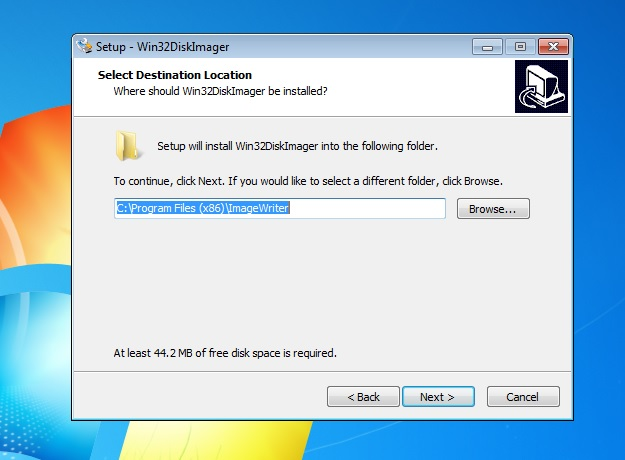
\includegraphics[width=0.5\textwidth]{Win32_2}
  	\end{center}
  	\caption{Win32DiskImager installation process part 2}
	\label{fig:2}
\end{figure}
Next on figure~\ref{fig:3} choose the Start Menu directory and select "Next".
\begin{figure}[H]
  	\begin{center}
    	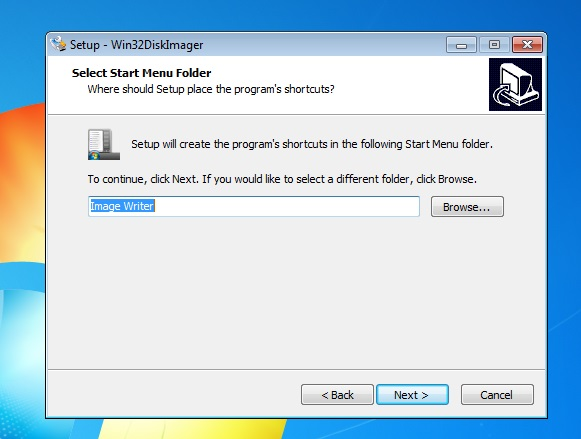
\includegraphics[width=0.5\textwidth]{Win32_3}
  	\end{center}
  	\caption{Win32DiskImager installation process part 3}
	\label{fig:3}
\end{figure}
Next on figure~\ref{fig:4} this window gives the option to create a desktop short cut by checking the check box. Select "Next".
\begin{figure}[H]
  	\begin{center}
    	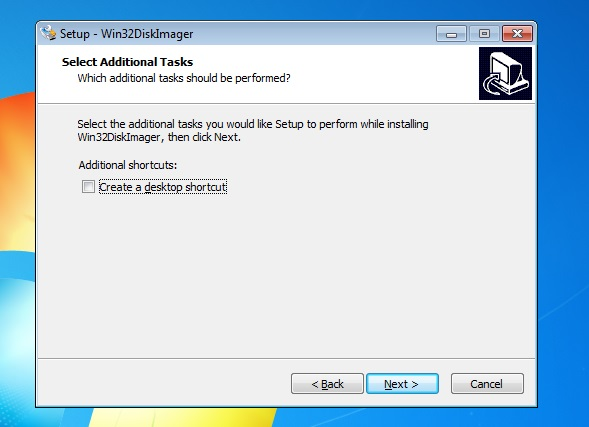
\includegraphics[width=0.5\textwidth]{Win32_4}
  	\end{center}
  	\caption{Win32DiskImager installation process part 4}
	\label{fig:4}
\end{figure}
Next on figure~\ref{fig:5} verify all the details are correct and select "Next".
\begin{figure}[H]
  	\begin{center}
    	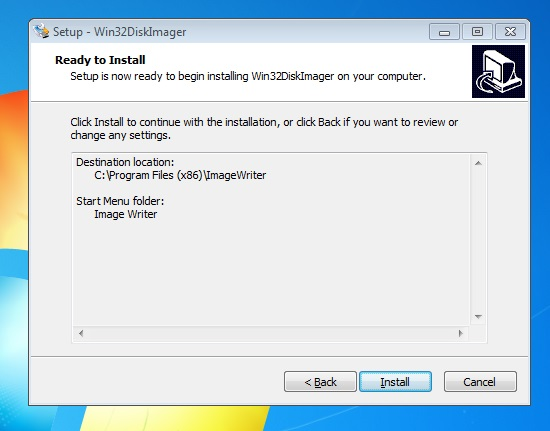
\includegraphics[width=0.5\textwidth]{Win32_5}
  	\end{center}
  	\caption{Win32DiskImager installation process part 5}
	\label{fig:5}
\end{figure}
Next on figure~\ref{fig:6} choose choose to "Launch Win32DiskImager" and select "Finish".
\begin{figure}[H]
  	\begin{center}
    	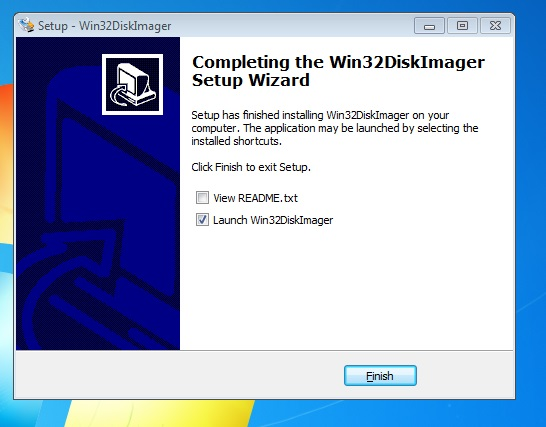
\includegraphics[width=0.5\textwidth]{Win32_6}
  	\end{center}
  	\caption{Win32DiskImager installation process part 6}
	\label{fig:6}
\end{figure}
Next on a window will open as shown on figure~\ref{fig:7} Select the folder icon to browse for image files.
\begin{figure}[H]
  	\begin{center}
    	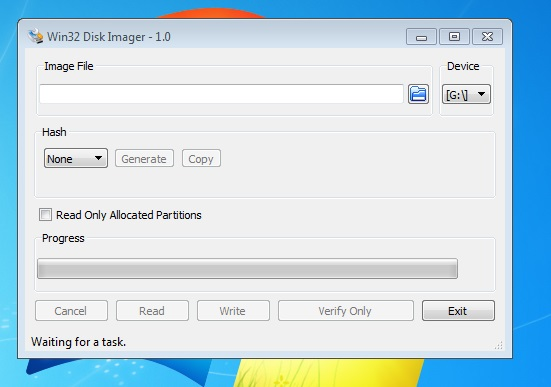
\includegraphics[width=0.5\textwidth]{Win32_7}
  	\end{center}
  	\caption{Debian Jessie installation process part 1}
	\label{fig:7}
\end{figure}
Nawigate to the image file as shown on figure~\ref{fig:8} In this case the image file is located in the /Instalation Files and Required Software directory. Select the image file and click "Open".
\begin{figure}[H]
  	\begin{center}
    	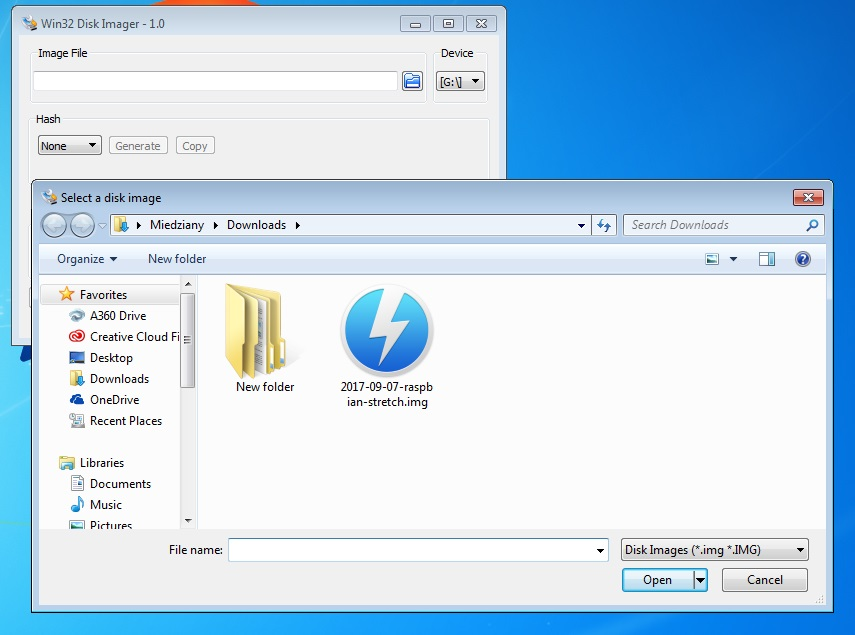
\includegraphics[width=0.5\textwidth]{Win32_8}
  	\end{center}
  	\caption{Debian Jessie installation process part 2}
	\label{fig:8}
\end{figure}
Select the micro SD card drive as shown on figure~\ref{fig:9}.
\begin{figure}[H]
  	\begin{center}
    	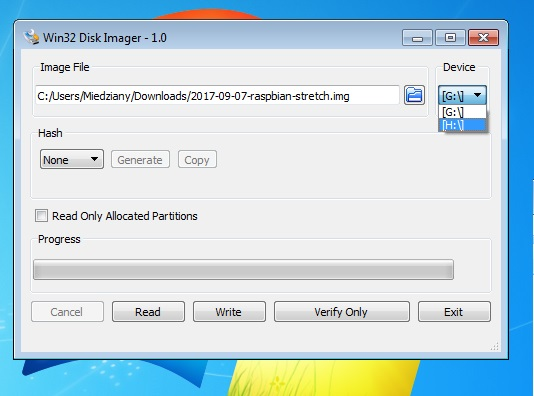
\includegraphics[width=0.5\textwidth]{Win32_9}
  	\end{center}
  	\caption{Debian Jessie installation process part 3}
	\label{fig:9}
\end{figure}
Select "Yes" as shown on figure~\ref{fig:10}.
\begin{figure}[H]
  	\begin{center}
    	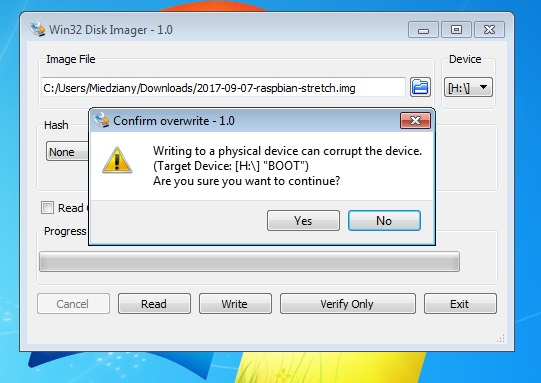
\includegraphics[width=0.5\textwidth]{Win32_10}
  	\end{center}
  	\caption{Debian Jessie installation process part 4}
	\label{fig:10}
\end{figure}
Figure~\ref{fig:11} shows what the writing of the image file to the micro SD card looks like.
\begin{figure}[H]
  	\begin{center}
    	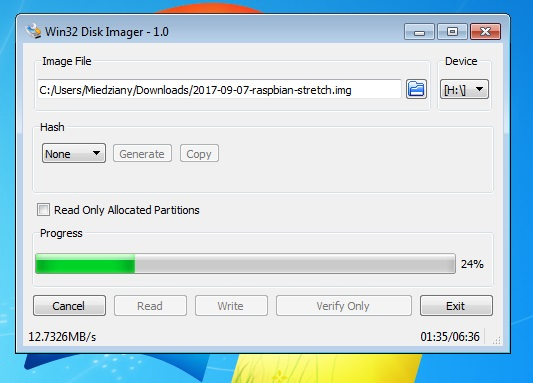
\includegraphics[width=0.5\textwidth]{Win32_11}
  	\end{center}
  	\caption{Debian Jessie installation process part 5}
	\label{fig:11}
\end{figure}
As shown on figure~\ref{fig:12} this pop up message will display once the writing of the image file has been completed.
\begin{figure}[H]
  	\begin{center}
    	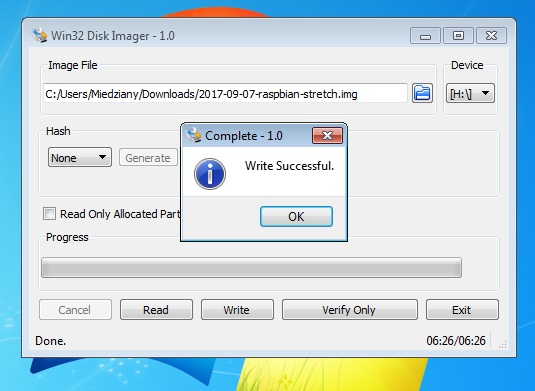
\includegraphics[width=0.5\textwidth]{Win32_12}
  	\end{center}
  	\caption{Debian Jessie installation process part 6}
	\label{fig:16}
\end{figure}
This concludes a successfully installation of Debian Jessie.\\
\textbf{Debian Jessie configuration}\\
In order to run the Raspberry Pi Jessie headless SSH has to be enabled.
Create a new text file as shown by figure~\ref{fig:20}, and select "Save As..." as shown by figure~\ref{fig:17}.
\begin{figure}[H]
  	\begin{center}
    	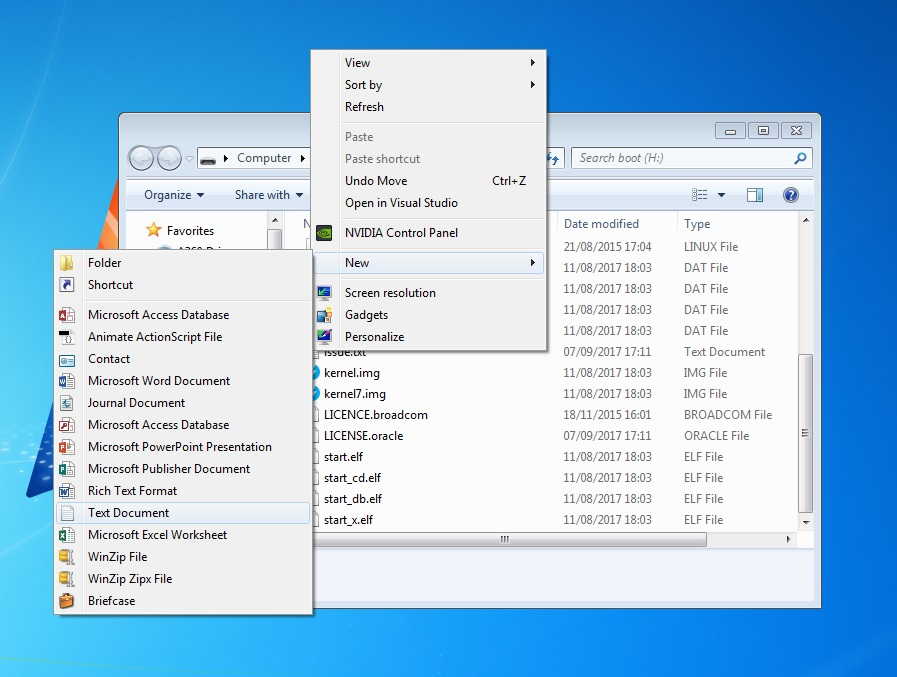
\includegraphics[width=0.9\textwidth]{Ras_1}
  	\end{center}
  	\caption{Debian Jessie configuration part 0}
	\label{fig:20}
\end{figure}
\begin{figure}[H]
  	\begin{center}
    	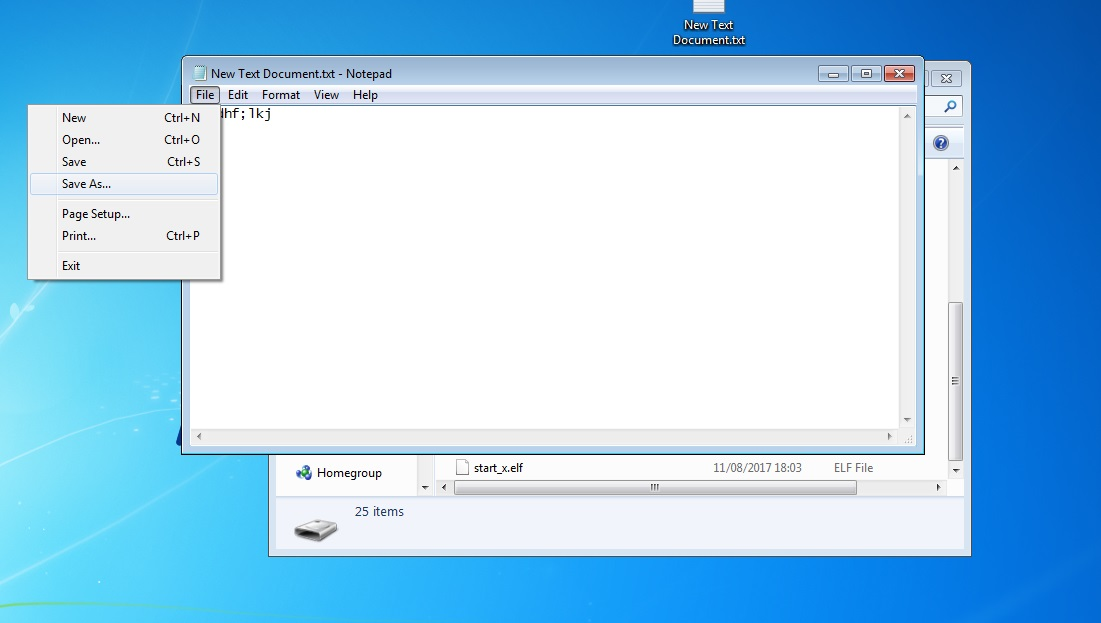
\includegraphics[width=0.9\textwidth]{Ras_1,1}
  	\end{center}
  	\caption{Debian Jessie configuration part 1}
	\label{fig:17}
\end{figure}
Select type as "All Files", and the file name "ssh" as shown by figure~\ref{fig:18}.
\begin{figure}[H]
  	\begin{center}
    	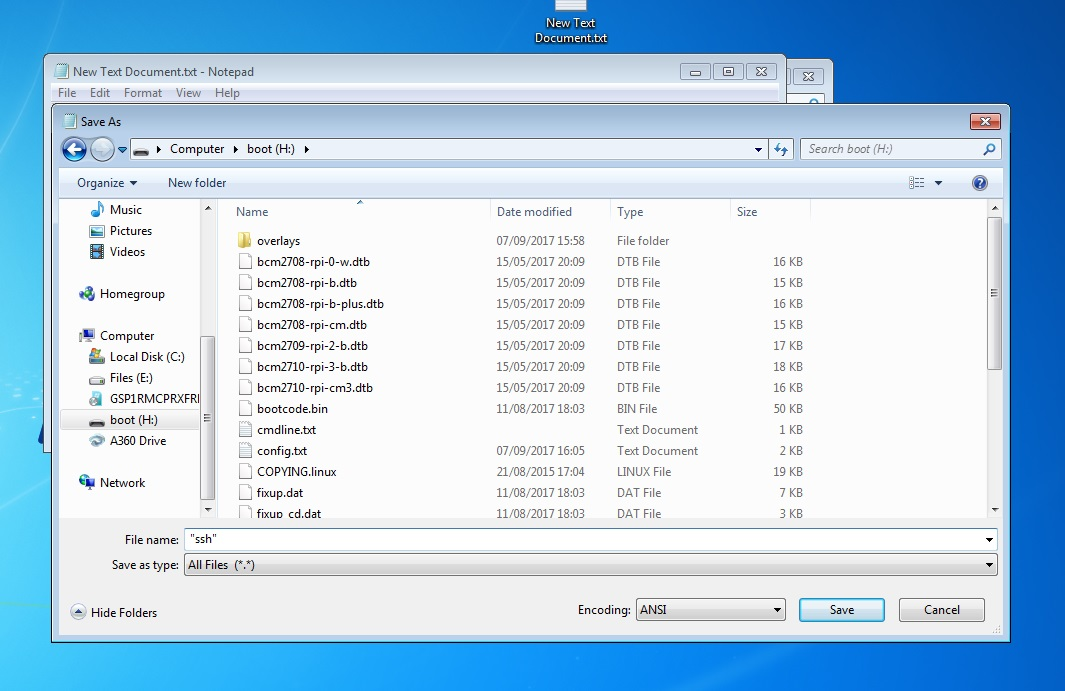
\includegraphics[width=0.9\textwidth]{Ras_1,2}
  	\end{center}
  	\caption{Debian Jessie configuration part 2}
	\label{fig:18}
\end{figure}
Figure~\ref{fig:19} shows what the micro SD card directory should look like after the ssh file has been copied to the drive.
\begin{figure}[H]
  	\begin{center}
    	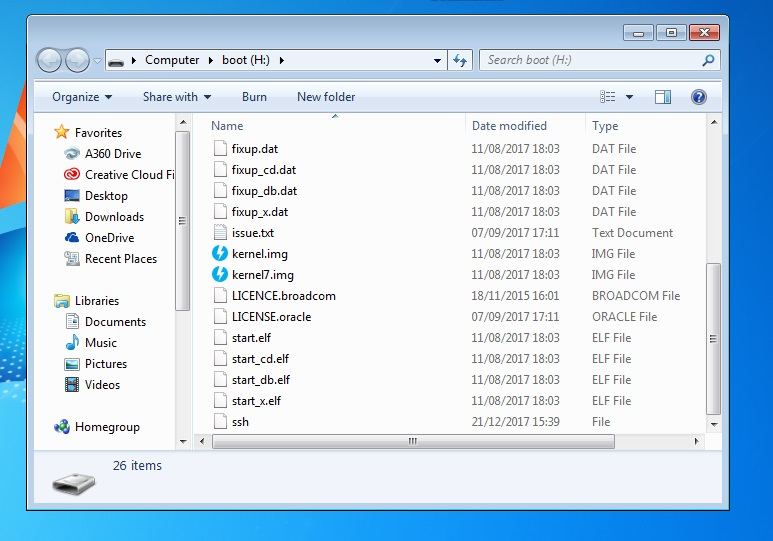
\includegraphics[width=0.9\textwidth]{Ras_1,3}
  	\end{center}
  	\caption{Debian Jessie configuration part 3}
	\label{fig:19}
\end{figure}
Connect Raspberry pi to the router and go to the router con-fig web page as shown by figure~\ref{fig:21}, and log into the router.
\begin{figure}[H]
  	\begin{center}
    	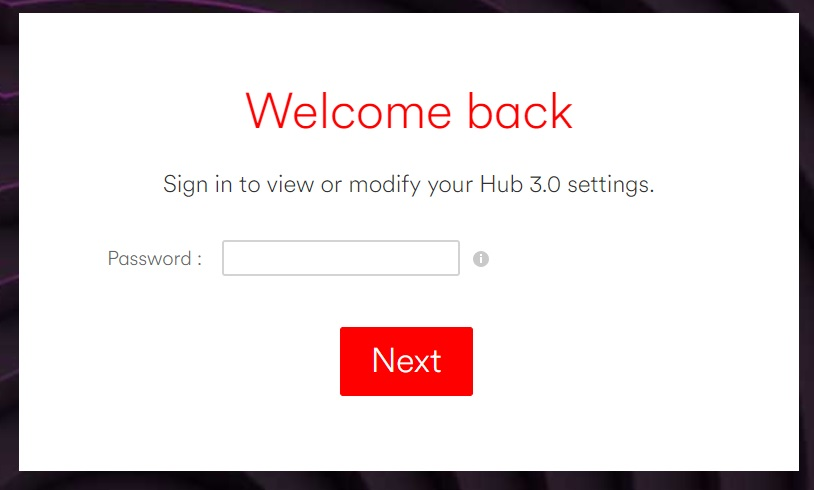
\includegraphics[width=0.9\textwidth]{Ras_3}
  	\end{center}
  	\caption{Debian Jessie configuration part 4}
	\label{fig:21}
\end{figure}
Select "Connected Devices" as shown by figure~\ref{fig:22}.
\begin{figure}[H]
  	\begin{center}
    	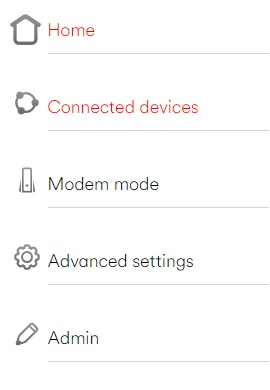
\includegraphics[width=0.9\textwidth]{Ras_4}
  	\end{center}
  	\caption{Debian Jessie configuration part 5}
	\label{fig:22}
\end{figure}
Raspberry Pi IP address can be seen as shown by figure~\ref{fig:23}.
\begin{figure}[H]
  	\begin{center}
    	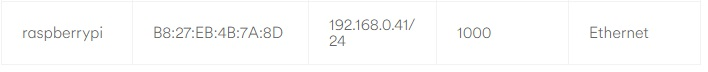
\includegraphics[width=0.9\textwidth]{Ras_5}
  	\end{center}
  	\caption{Debian Jessie configuration part 6}
	\label{fig:23}
\end{figure}
Next open the Putty terminal located in the /Instalation Files and Required Software directory, and enter Raspberry PI IP address as shown by figure~\ref{fig:24}. And click "Open".
\begin{figure}[H]
  	\begin{center}
    	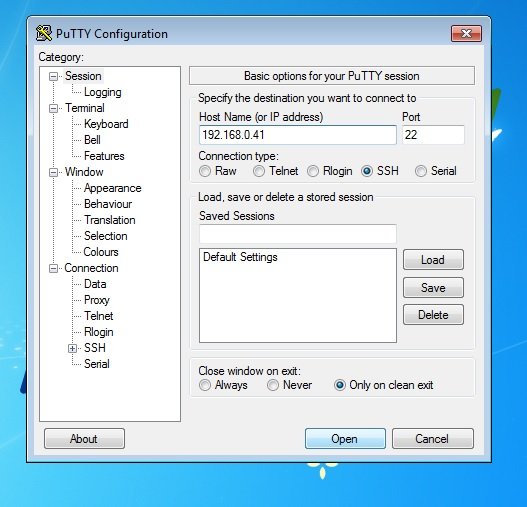
\includegraphics[width=0.9\textwidth]{Ras_6}
  	\end{center}
  	\caption{Debian Jessie configuration part 7}
	\label{fig:24}
\end{figure}
On the pop up window select "Yes" as shown by figure~\ref{fig:25}.
\begin{figure}[H]
  	\begin{center}
    	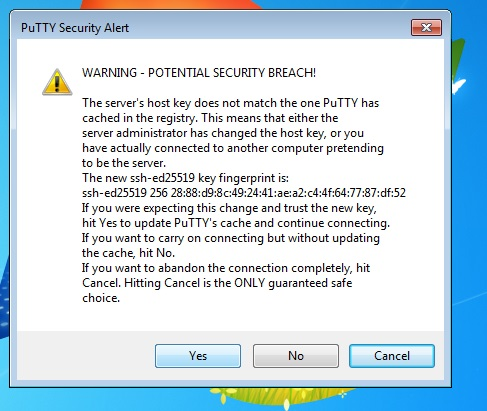
\includegraphics[width=0.9\textwidth]{Ras_7}
  	\end{center}
  	\caption{Debian Jessie configuration part 8}
	\label{fig:25}
\end{figure}
Next the terminal will ask for user-name, type "pi" and then the terminal will ask for the password, type "raspberry". This will result in a successful log in, as shown by figure~\ref{fig:26}.
\begin{figure}[H]
  	\begin{center}
    	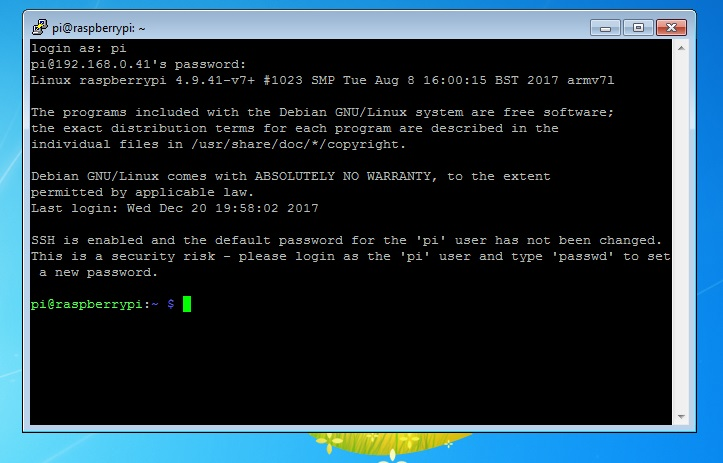
\includegraphics[width=0.9\textwidth]{Ras_8}
  	\end{center}
  	\caption{Debian Jessie configuration part 9}
	\label{fig:26}
\end{figure}
Next enter "sudo raspi-config" as shown by figure~\ref{fig:27}.
\begin{figure}[H]
  	\begin{center}
    	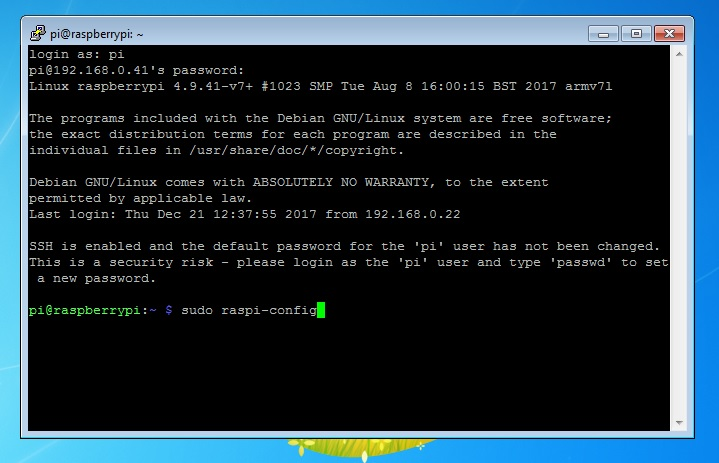
\includegraphics[width=0.9\textwidth]{Ras_9}
  	\end{center}
  	\caption{Debian Jessie configuration part 10}
	\label{fig:27}
\end{figure}
Navigate to "Advanced Options" as shown by figure~\ref{fig:28}.
\begin{figure}[H]
  	\begin{center}
    	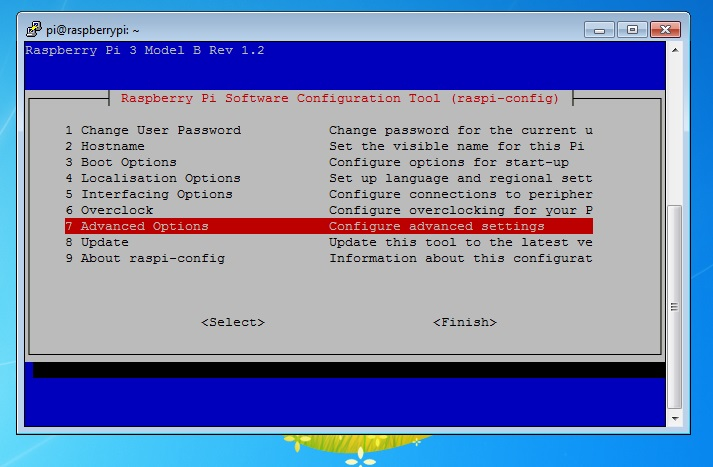
\includegraphics[width=0.9\textwidth]{Ras_10}
  	\end{center}
  	\caption{Debian Jessie configuration part 11}
	\label{fig:28}
\end{figure}
And select "Expand Filesystem" as shown by figure~\ref{fig:29}.
\begin{figure}[H]
  	\begin{center}
    	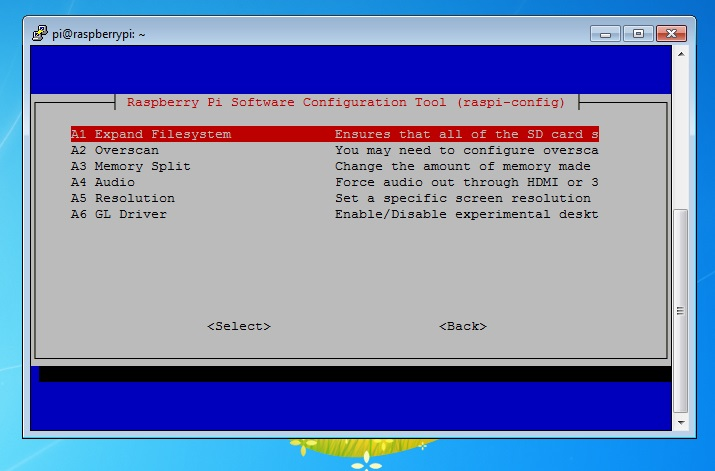
\includegraphics[width=0.9\textwidth]{Ras_11}
  	\end{center}
  	\caption{Debian Jessie configuration part 12}
	\label{fig:29}
\end{figure}
Select "OK" as shown by figure~\ref{fig:30}.
\begin{figure}[H]
  	\begin{center}
    	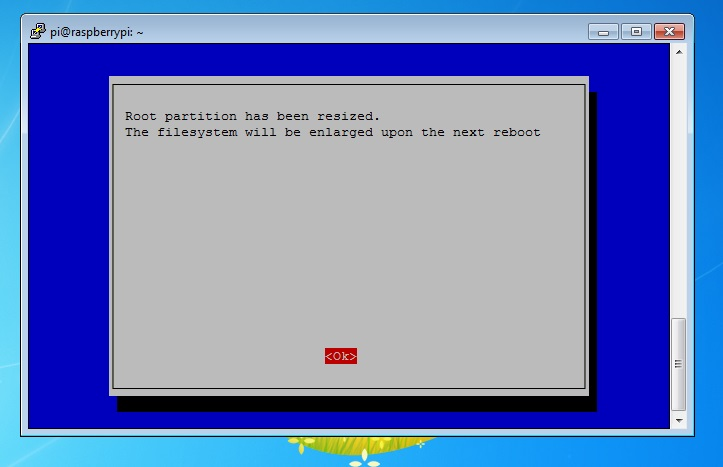
\includegraphics[width=0.9\textwidth]{Ras_12}
  	\end{center}
  	\caption{Debian Jessie configuration part 13}
	\label{fig:30}
\end{figure}
Select "Finish" as shown by figure~\ref{fig:31}.
\begin{figure}[H]
  	\begin{center}
    	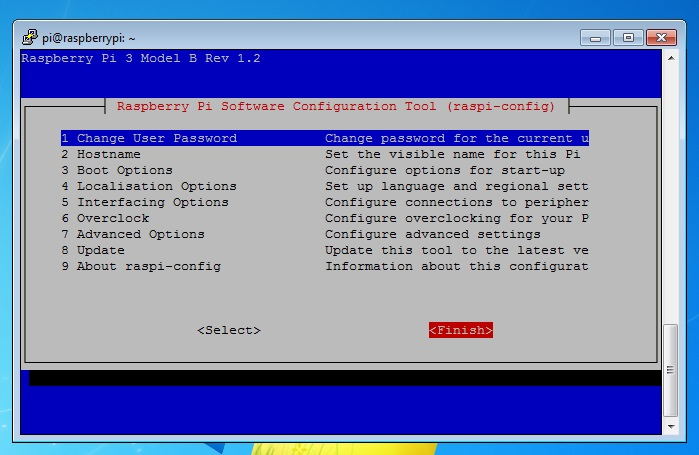
\includegraphics[width=0.9\textwidth]{Ras_13}
  	\end{center}
  	\caption{Debian Jessie configuration part 14}
	\label{fig:31}
\end{figure}
Select "Yes" as shown by figure~\ref{fig:32}.
\begin{figure}[H]
  	\begin{center}
    	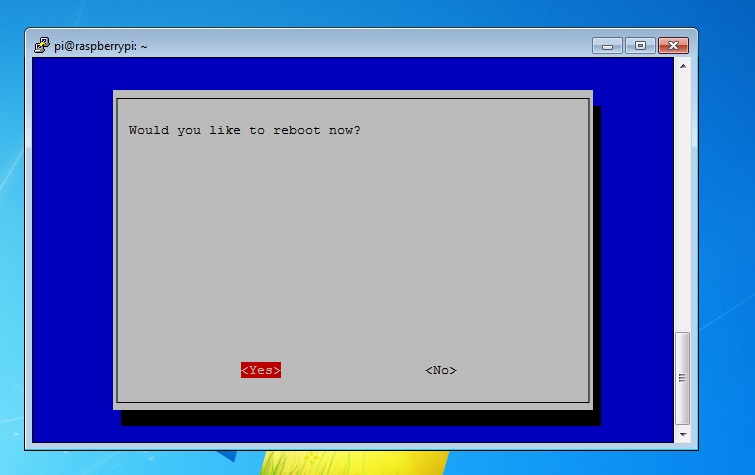
\includegraphics[width=0.9\textwidth]{Ras_14}
  	\end{center}
  	\caption{Debian Jessie configuration part 15}
	\label{fig:32}
\end{figure}
This will close the connection with the Server as shown by figure~\ref{fig:33}.
\begin{figure}[H]
  	\begin{center}
    	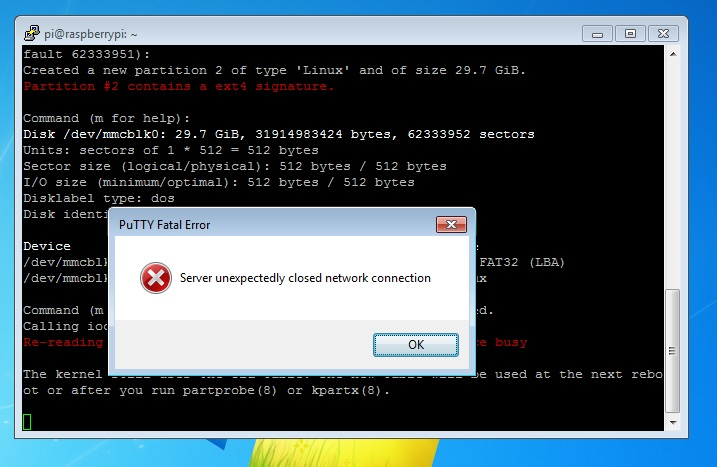
\includegraphics[width=0.9\textwidth]{Ras_15}
  	\end{center}
  	\caption{Debian Jessie configuration part 16}
	\label{fig:33}
\end{figure}
Restart the putty connection repeating the process from part 7. Next type "sudo apt-get update" as shown by figure~\ref{fig:34}. This will update the software and all the repositories.
\begin{figure}[H]
  	\begin{center}
    	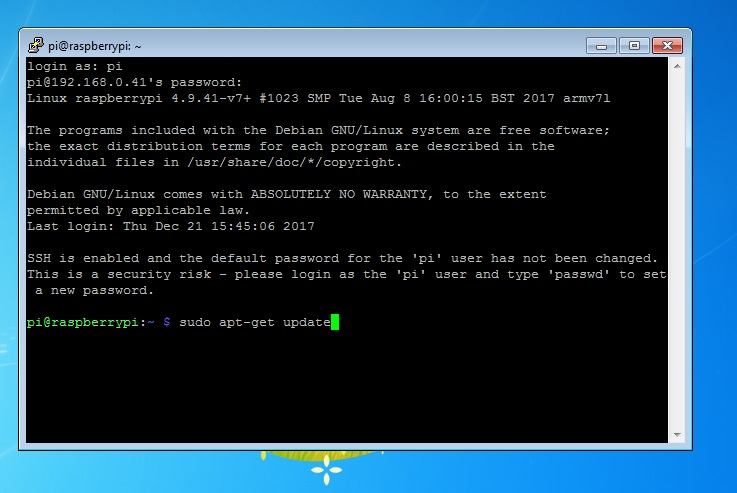
\includegraphics[width=0.9\textwidth]{Ras_16}
  	\end{center}
  	\caption{Debian Jessie configuration part 17}
	\label{fig:34}
\end{figure}
This will take some time. Next type "sudo apt-get dist-upgrade" the terminal will look like figure~\ref{fig:35}. This will update the software and all the repositories.
\begin{figure}[H]
  	\begin{center}
    	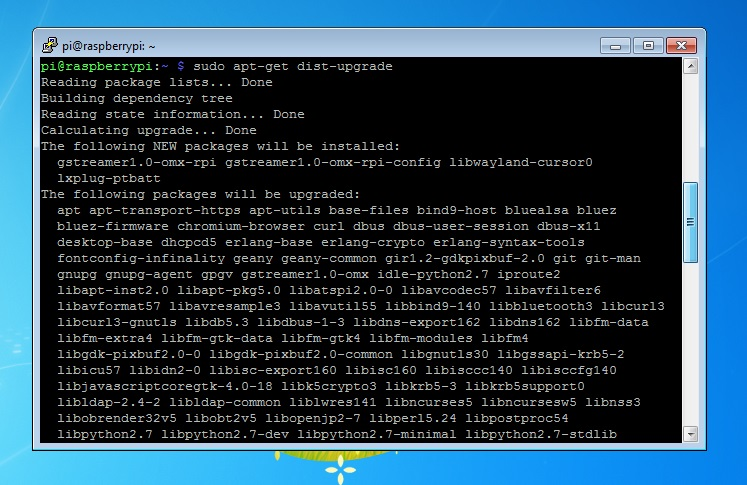
\includegraphics[width=0.9\textwidth]{Ras_17}
  	\end{center}
  	\caption{Debian Jessie configuration part 18}
	\label{fig:35}
\end{figure}
Next install Apache web server by typing the following command "sudo apt-get install apache2 -y" figure~\ref{fig:36}.
\begin{figure}[H]
  	\begin{center}
    	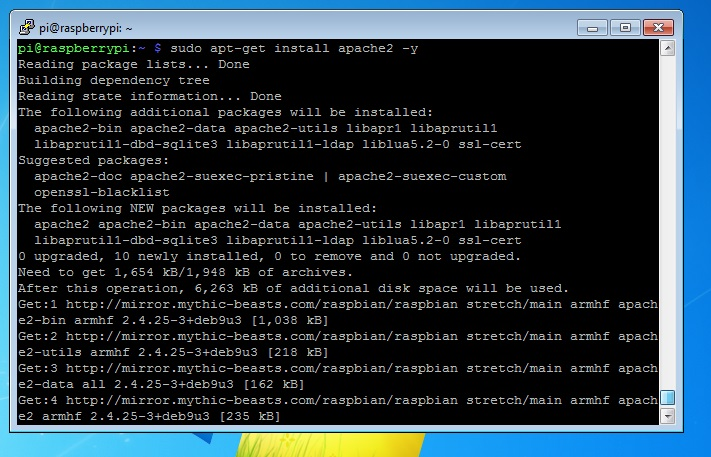
\includegraphics[width=0.9\textwidth]{Ras_18}
  	\end{center}
  	\caption{MariaDB instalation part 1}
	\label{fig:36}
\end{figure}
After the sucessfull instalation of Apache web server, by entering Raspberry PI IP into the browser, the browser should look like figure~\ref{fig:37}.
\begin{figure}[H]
  	\begin{center}
    	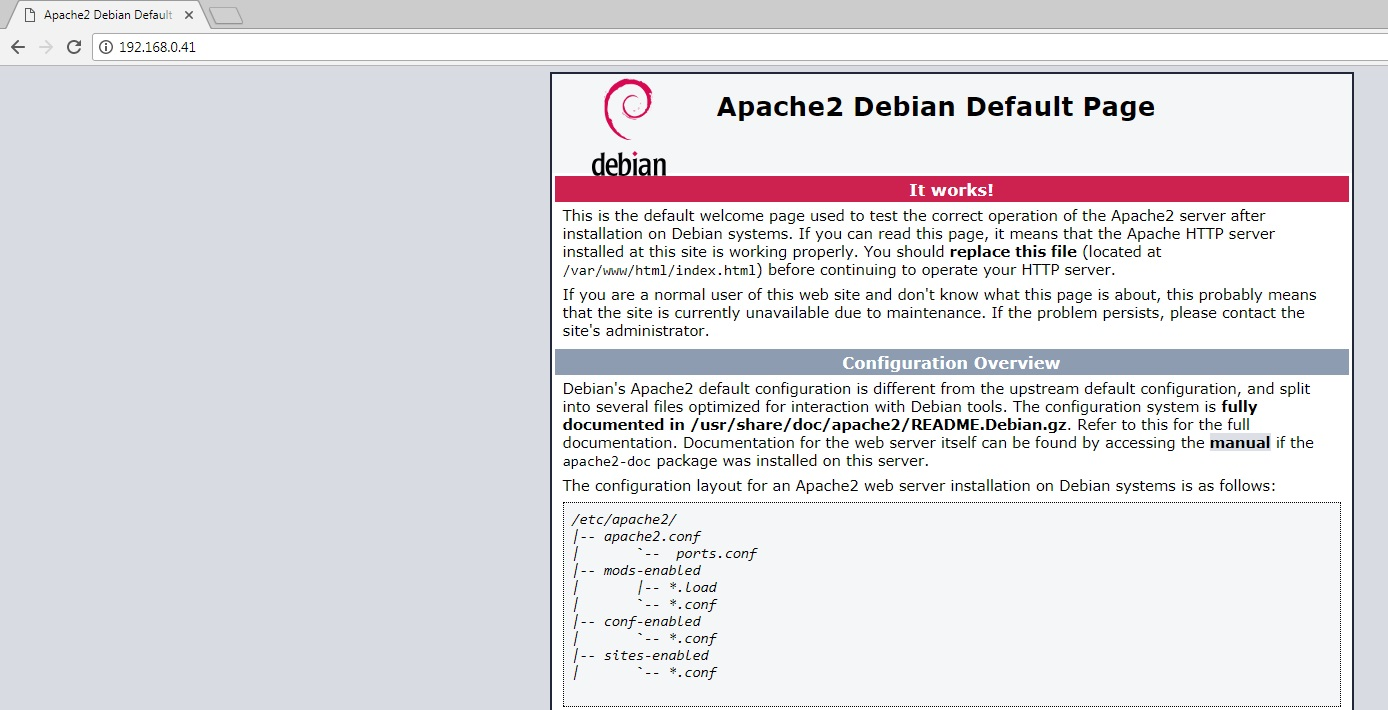
\includegraphics[width=0.9\textwidth]{Ras_19}
  	\end{center}
  	\caption{MariaDB instalation part 2}
	\label{fig:37}
\end{figure}
Next install PHP with the command "sudo apt-get install php" as show by figure~\ref{fig:38}.
\begin{figure}[H]
  	\begin{center}
    	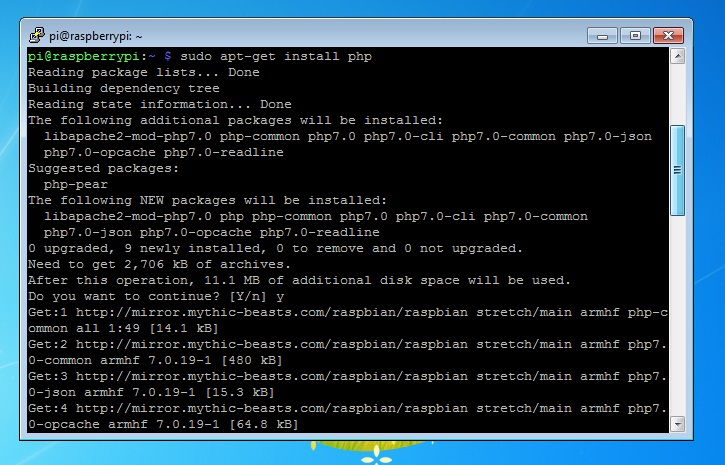
\includegraphics[width=0.9\textwidth]{Ras_20}
  	\end{center}
  	\caption{MariaDB instalation part 3}
	\label{fig:38}
\end{figure}
Next install MySQL Server with the command "sudo apt-get install mysql-server -y" as show by figure~\ref{fig:39}.
\begin{figure}[H]
  	\begin{center}
    	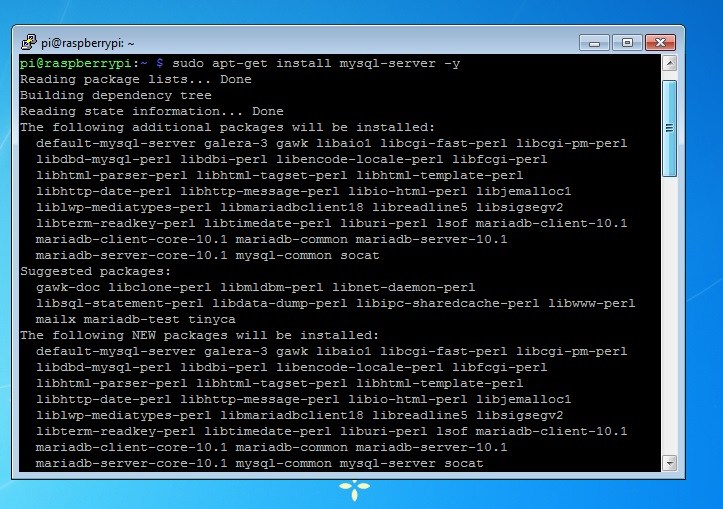
\includegraphics[width=0.9\textwidth]{Ras_21}
  	\end{center}
  	\caption{MariaDB instalation part 4}
	\label{fig:39}
\end{figure}
Next install MySQL Client with the command "sudo apt-get install mysql-client -y" as show by figure~\ref{fig:40}.
\begin{figure}[H]
  	\begin{center}
    	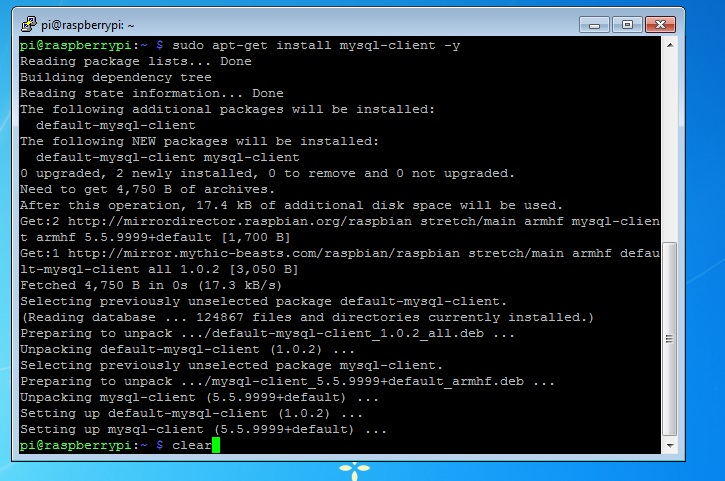
\includegraphics[width=0.9\textwidth]{Ras_22}
  	\end{center}
  	\caption{MariaDB instalation part 5}
	\label{fig:40}
\end{figure}
Next install MySQL  repository for PHP with the command "sudo apt-get install php-mysql -y" as show by figure~\ref{fig:41}.
\begin{figure}[H]
  	\begin{center}
    	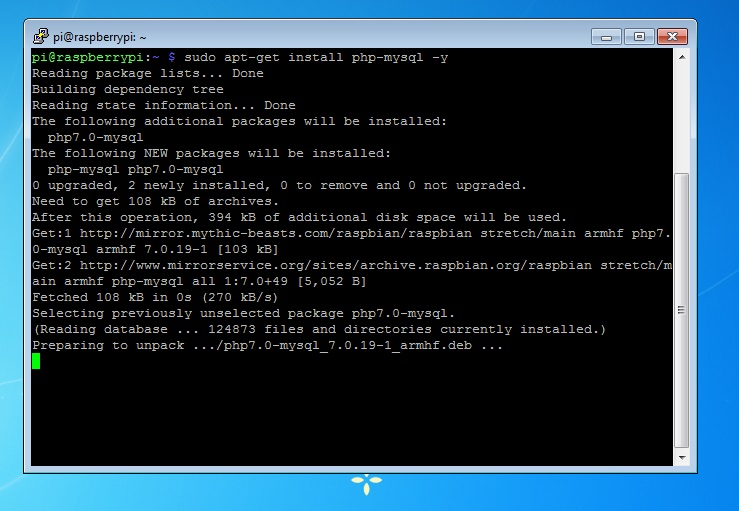
\includegraphics[width=0.9\textwidth]{Ras_23}
  	\end{center}
  	\caption{MariaDB instalation part 6}
	\label{fig:41}
\end{figure}
Log into MySQL using "root" as user as show by figure~\ref{fig:42}. When the terminal asks for password just click "Enter" as the root user after installation has no password.
\begin{figure}[H]
  	\begin{center}
    	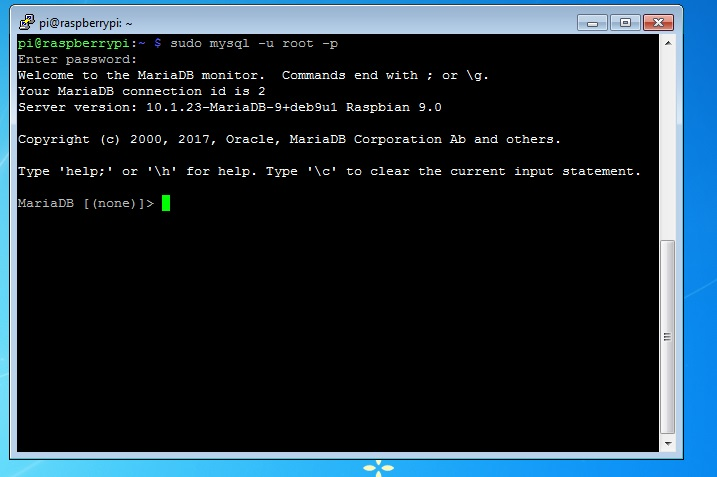
\includegraphics[width=0.9\textwidth]{Ras_24}
  	\end{center}
  	\caption{Database configuration part 1}
	\label{fig:42}
\end{figure}
This is an optional step to create a password for the root user as show by figure~\ref{fig:43}. This will increase server security. Exit the server and restart it by typing "sudo service mysql restart" and then login to the server using the new password as show by figure~\ref{fig:44}.
\begin{figure}[H]
  	\begin{center}
    	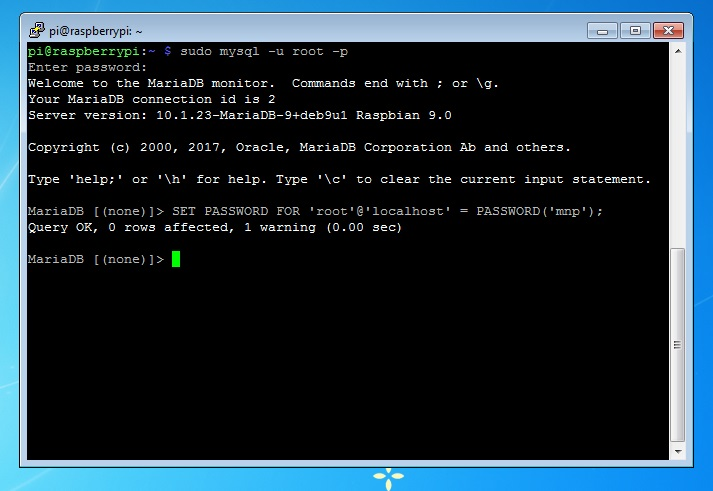
\includegraphics[width=0.9\textwidth]{Ras_25}
  	\end{center}
  	\caption{Database configuration part 2}
	\label{fig:43}
\end{figure}
\begin{figure}[H]
  	\begin{center}
    	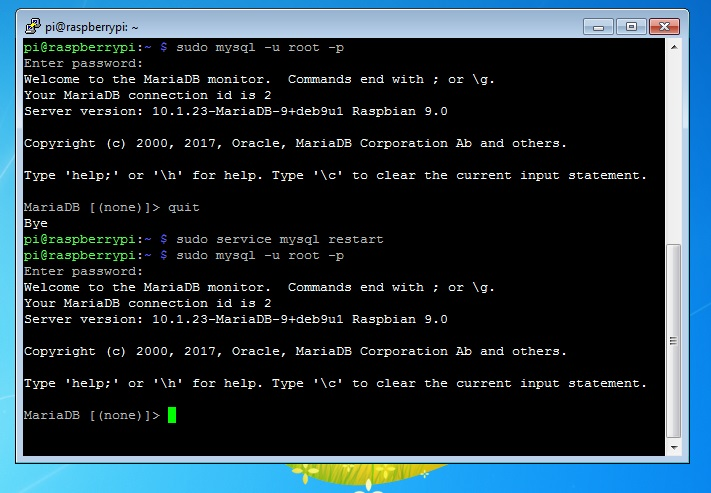
\includegraphics[width=0.9\textwidth]{Ras_26}
  	\end{center}
  	\caption{Database configuration part 3}
	\label{fig:44}
\end{figure}
Create the "ecgpedodata" database as show by figure~\ref{fig:45}.
\begin{figure}[H]
  	\begin{center}
    	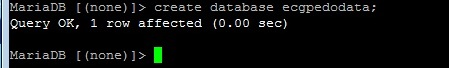
\includegraphics[width=0.9\textwidth]{Ras_29}
  	\end{center}
  	\caption{Database configuration part 4}
	\label{fig:45}
\end{figure}
Change the current database by using the command "USE ecgpedodata" as show by figure~\ref{fig:46}.
\begin{figure}[H]
  	\begin{center}
    	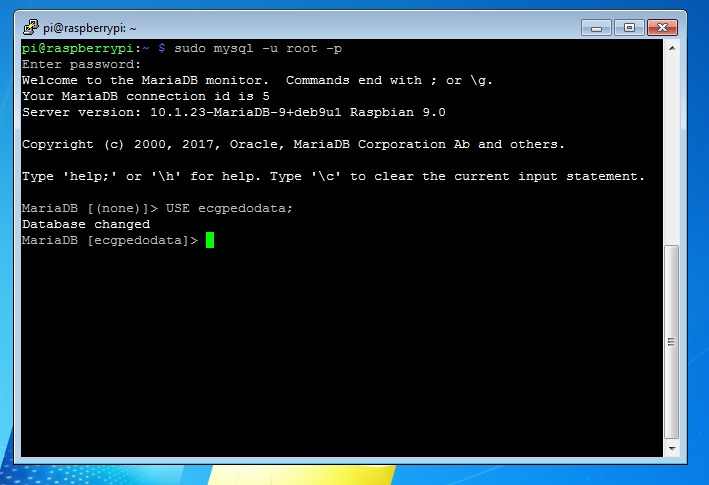
\includegraphics[width=0.9\textwidth]{Ras_30}
  	\end{center}
  	\caption{Database configuration part 5}
	\label{fig:46}
\end{figure}
Create table "patien1" as show by figure~\ref{fig:47}.
\begin{figure}[H]
  	\begin{center}
    	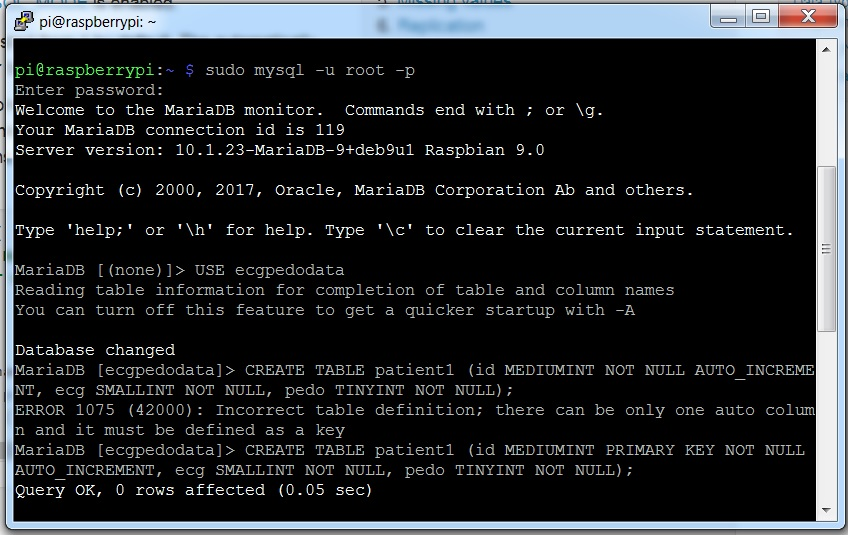
\includegraphics[width=0.9\textwidth]{Ras_31}
  	\end{center}
  	\caption{Database configuration part 6}
	\label{fig:47}
\end{figure}
Use the INSERT command to enter data into the table as show by figure~\ref{fig:48}.
\begin{figure}[H]
  	\begin{center}
    	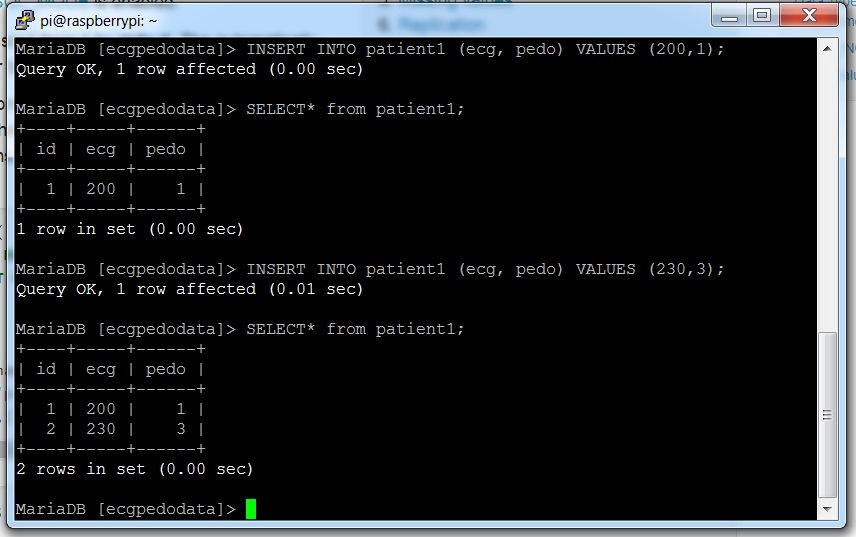
\includegraphics[width=0.9\textwidth]{Ras_32}
  	\end{center}
  	\caption{Database configuration part 7}
	\label{fig:48}
\end{figure}
Create a new user that will have access to ecgpedodata database from local-host as show by figure~\ref{fig:49}.
\begin{figure}[H]
  	\begin{center}
    	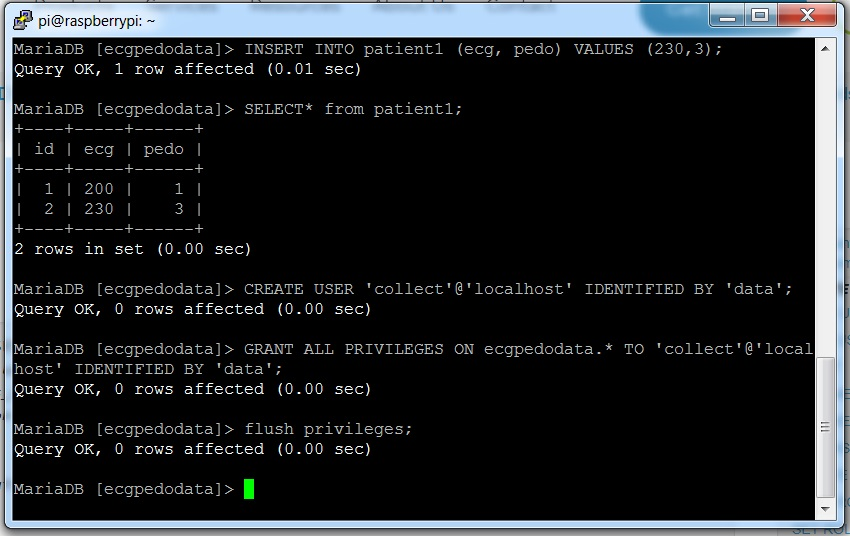
\includegraphics[width=0.9\textwidth]{Ras_33}
  	\end{center}
  	\caption{Database configuration part 8}
	\label{fig:49}
\end{figure}
Exit the database and navigate as superuser to /var/www/html/ direcotry using cd command as show by figure~\ref{fig:50}.
\begin{figure}[H]
  	\begin{center}
    	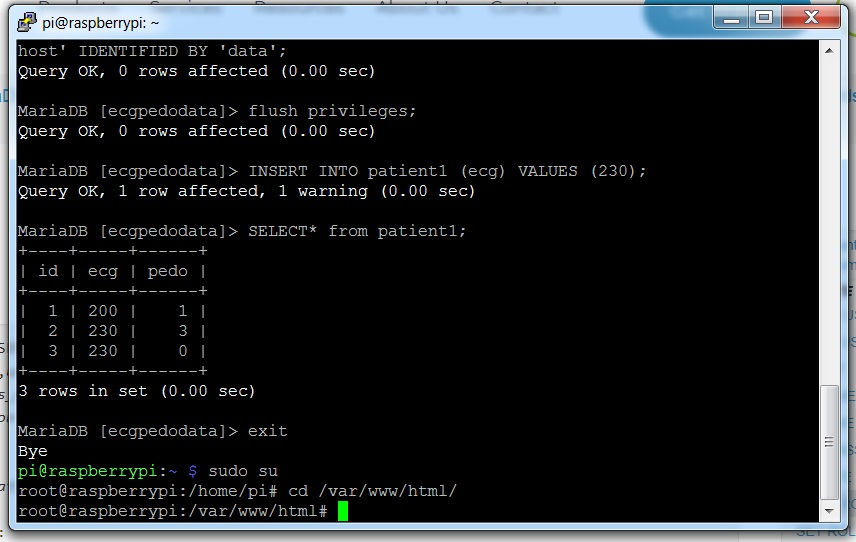
\includegraphics[width=0.9\textwidth]{Ras_34}
  	\end{center}
  	\caption{PHP file configuration part 1}
	\label{fig:50}
\end{figure}
Create a 'collectdata.php' file using nano editor as show by figure~\ref{fig:51}.
\begin{figure}[H]
  	\begin{center}
    	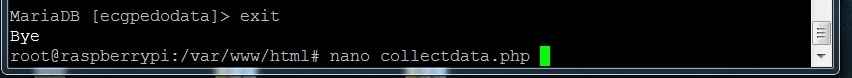
\includegraphics[width=0.9\textwidth]{Ras_35}
  	\end{center}
  	\caption{PHP file configuration part 2}
	\label{fig:51}
\end{figure}
Enter the PHP code as show by figure~\ref{fig:52}.
\begin{figure}[H]
  	\begin{center}
    	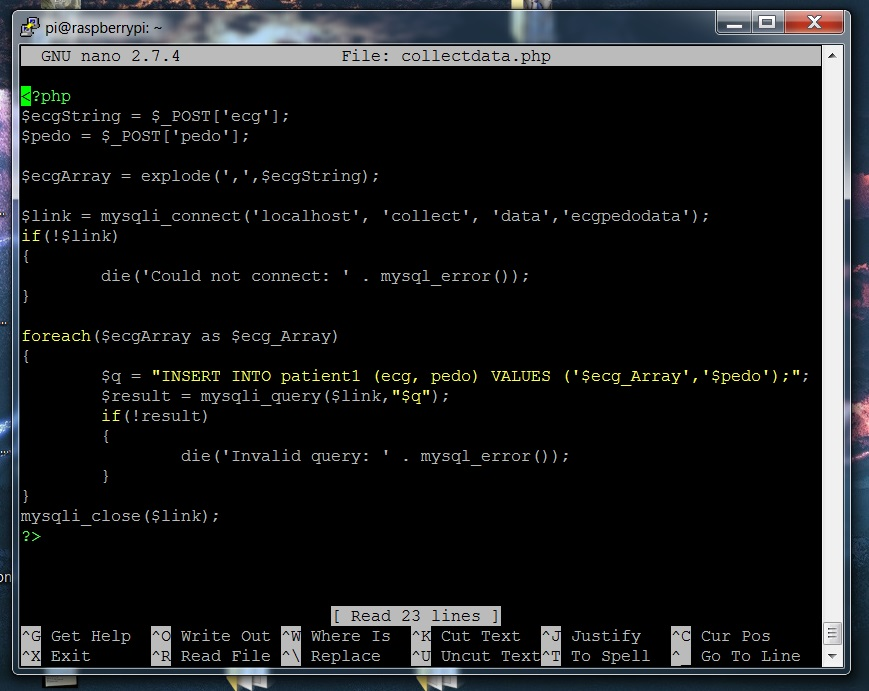
\includegraphics[width=0.9\textwidth]{Ras_36}
  	\end{center}
  	\caption{PHP file configuration part 3}
	\label{fig:52}
\end{figure}
Use an online POST generator to simulate POST request to collectdata.php as show by figure~\ref{fig:53}. And check if the values have been enterd into the table as shown by figure~\ref{fig:54}.
\begin{figure}[H]
  	\begin{center}
    	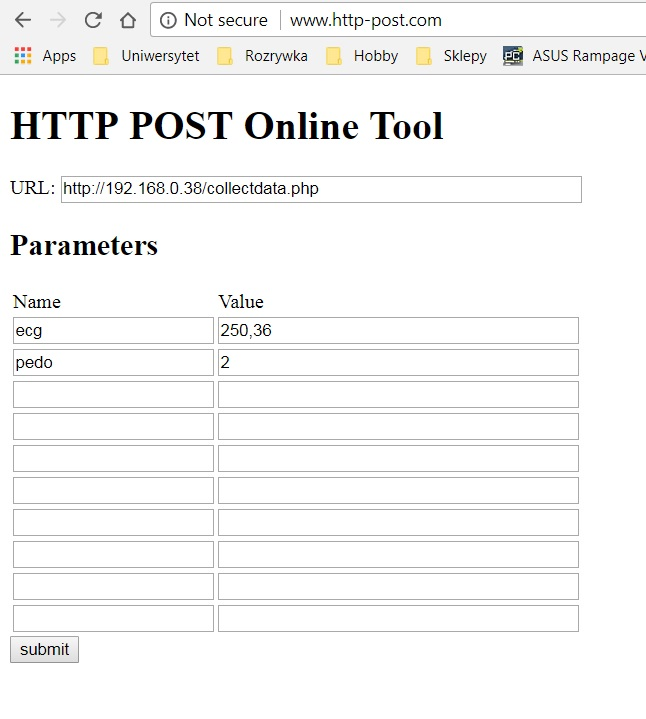
\includegraphics[width=0.9\textwidth]{Ras_38}
  	\end{center}
  	\caption{PHP file configuration part 4}
	\label{fig:53}
\end{figure}
\begin{figure}[H]
  	\begin{center}
    	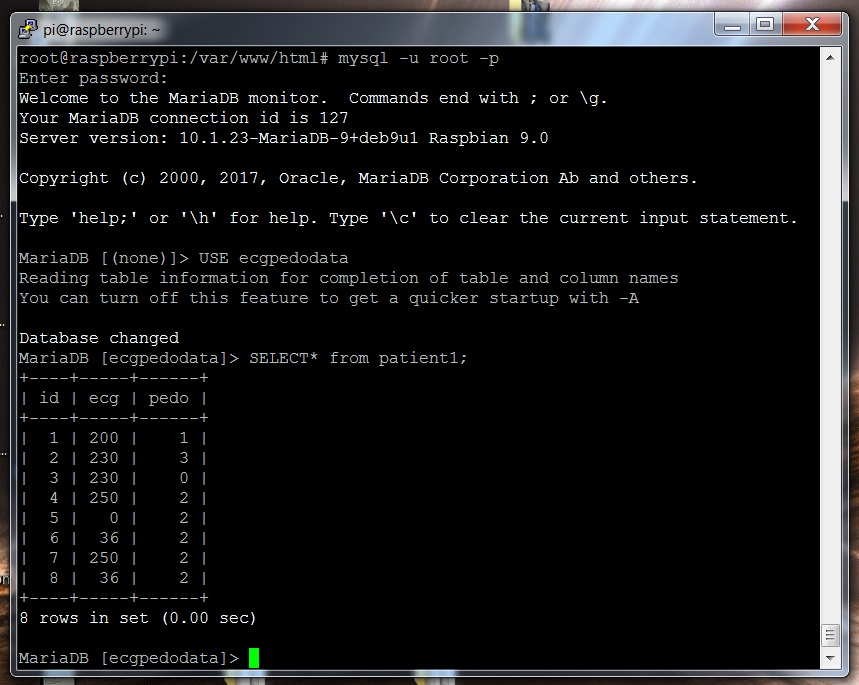
\includegraphics[width=0.9\textwidth]{Ras_37}
  	\end{center}
  	\caption{PHP file configuration part 5}
	\label{fig:54}
\end{figure}
Create a new user that will be able to log into the server remotely as shown by figure~\ref{fig:55}. And grant all privalages to the new user but at an IP adress not a localhost as shown by figure~\ref{fig:56}.
\begin{figure}[H]
  	\begin{center}
    	\includegraphics[width=0.9\textwidth]{Ras_39}
  	\end{center}
  	\caption{Web application user creation part 1}
	\label{fig:55}
\end{figure}
\begin{figure}[H]
  	\begin{center}
    	\includegraphics[width=0.9\textwidth]{Ras_40}
  	\end{center}
  	\caption{Web application user creation part 2}
	\label{fig:56}
\end{figure}
This concludes the Raspberry Pi 3 set-up.
\end{document}
